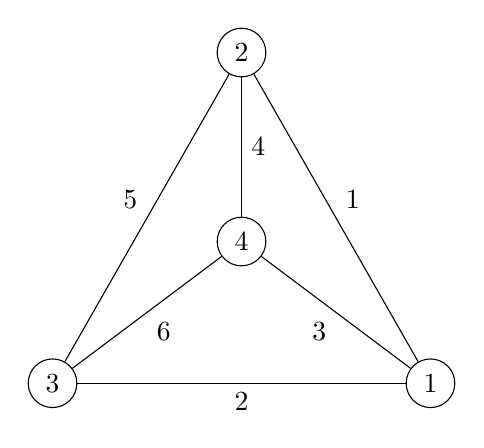
\begin{tikzpicture}
	\begin{scope}[xshift=0cm, yshift=0cm, scale=0.6]
		\node[circle, draw] (1) at (4, -3) {1};
		\node[circle, draw] (2) at (0, 4) {2};
		\node[circle, draw] (3) at (-4, -3) {3};
		\node[circle, draw] (4) at (0, 0) {4};
	
		\draw[draw] (1) -- node[above right] {1} (2);
		\draw[draw] (1) -- node[below] {2} (3);
		\draw[draw] (1) -- node[below left] {3} (4);
		\draw[draw] (2) -- node[right] {4} (4);
		\draw[draw] (2) -- node[above left] {5} (3);
		\draw[draw] (3) -- node[below right] {6} (4);
	\end{scope}
\end{tikzpicture}